\begin{figure}[H]
\centering
\resizebox{\columnwidth}{!}{%
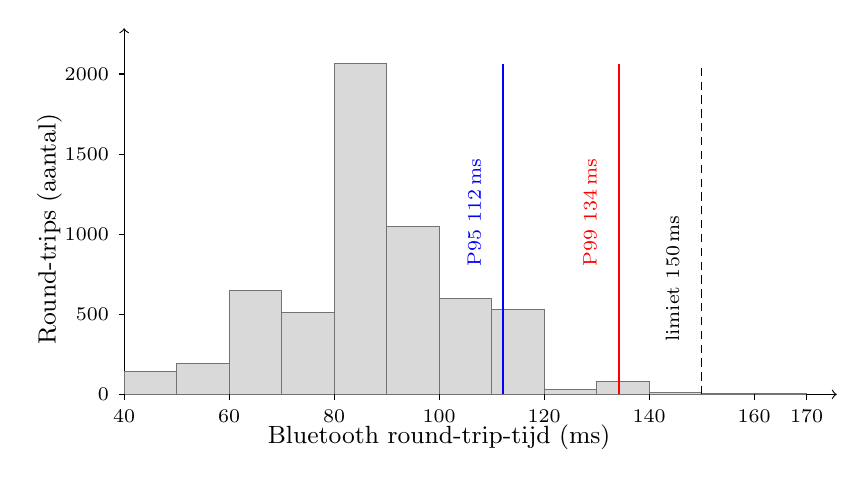
\begin{tikzpicture}
\draw[->] (-0.05,0) -- (9.05,0);
\draw[->] (0,0) -- (0,4.65);
% --- bars ---
\fill[black!15] (0.000,0) rectangle (0.667,0.287);
\draw[black!55,line width=0.3pt] (0.000,0) rectangle (0.667,0.287);
\fill[black!15] (0.667,0) rectangle (1.333,0.393);
\draw[black!55,line width=0.3pt] (0.667,0) rectangle (1.333,0.393);
\fill[black!15] (1.333,0) rectangle (2.000,1.322);
\draw[black!55,line width=0.3pt] (1.333,0) rectangle (2.000,1.322);
\fill[black!15] (2.000,0) rectangle (2.667,1.041);
\draw[black!55,line width=0.3pt] (2.000,0) rectangle (2.667,1.041);
\fill[black!15] (2.667,0) rectangle (3.333,4.200);
\draw[black!55,line width=0.3pt] (2.667,0) rectangle (3.333,4.200);
\fill[black!15] (3.333,0) rectangle (4.000,2.136);
\draw[black!55,line width=0.3pt] (3.333,0) rectangle (4.000,2.136);
\fill[black!15] (4.000,0) rectangle (4.667,1.214);
\draw[black!55,line width=0.3pt] (4.000,0) rectangle (4.667,1.214);
\fill[black!15] (4.667,0) rectangle (5.333,1.074);
\draw[black!55,line width=0.3pt] (4.667,0) rectangle (5.333,1.074);
\fill[black!15] (5.333,0) rectangle (6.000,0.063);
\draw[black!55,line width=0.3pt] (5.333,0) rectangle (6.000,0.063);
\fill[black!15] (6.000,0) rectangle (6.667,0.165);
\draw[black!55,line width=0.3pt] (6.000,0) rectangle (6.667,0.165);
\fill[black!15] (6.667,0) rectangle (7.333,0.026);
\draw[black!55,line width=0.3pt] (6.667,0) rectangle (7.333,0.026);
\fill[black!15] (7.333,0) rectangle (8.000,0.014);
\draw[black!55,line width=0.3pt] (7.333,0) rectangle (8.000,0.014);
\fill[black!15] (8.000,0) rectangle (8.667,0.008);
\draw[black!55,line width=0.3pt] (8.000,0) rectangle (8.667,0.008);
% --- percentile + threshold lines ---
\draw[blue,thick] (4.816,0) -- (4.816,4.20); \node[blue,font=\scriptsize,rotate=90,anchor=south] at (4.656,2.31) {P95 112\,ms};
\draw[red,thick] (6.285,0) -- (6.285,4.20); \node[red,font=\scriptsize,rotate=90,anchor=south] at (6.125,2.31) {P99 134\,ms};
\draw[densely dashed] (7.333,0) -- (7.333,4.20); \node[font=\scriptsize,rotate=90,anchor=south] at (7.173,1.47) {limiet 150\,ms};
% --- x ticks ---
\draw (0.000,0) -- (0.000,-0.07); \node[below,font=\scriptsize] at (0.000,-0.07) {40};
\draw (1.333,0) -- (1.333,-0.07); \node[below,font=\scriptsize] at (1.333,-0.07) {60};
\draw (2.667,0) -- (2.667,-0.07); \node[below,font=\scriptsize] at (2.667,-0.07) {80};
\draw (4.000,0) -- (4.000,-0.07); \node[below,font=\scriptsize] at (4.000,-0.07) {100};
\draw (5.333,0) -- (5.333,-0.07); \node[below,font=\scriptsize] at (5.333,-0.07) {120};
\draw (6.667,0) -- (6.667,-0.07); \node[below,font=\scriptsize] at (6.667,-0.07) {140};
\draw (8.000,0) -- (8.000,-0.07); \node[below,font=\scriptsize] at (8.000,-0.07) {160};
\draw (8.667,0) -- (8.667,-0.07); \node[below,font=\scriptsize] at (8.667,-0.07) {170};
% --- y ticks (round) ---
\draw (-0.07,0.000) -- (0,0.000); \node[left,font=\scriptsize] at (-0.07,0.000) {0};
\draw (-0.07,1.017) -- (0,1.017); \node[left,font=\scriptsize] at (-0.07,1.017) {500};
\draw (-0.07,2.034) -- (0,2.034); \node[left,font=\scriptsize] at (-0.07,2.034) {1000};
\draw (-0.07,3.051) -- (0,3.051); \node[left,font=\scriptsize] at (-0.07,3.051) {1500};
\draw (-0.07,4.068) -- (0,4.068); \node[left,font=\scriptsize] at (-0.07,4.068) {2000};
\node[font=\small] at (4.00,-0.55) {Bluetooth round-trip-tijd (ms)};
\node[font=\small,rotate=90] at (-0.95,2.10) {Round-trips (aantal)};
\end{tikzpicture}%
}
\caption{Verdeling van de Bluetooth round-trip-tijden over campagne 2 (n=5872, bins van 10\,ms). De vooraf geregistreerde DV1(b)-drempels zijn P95 $<$ 150\,ms en P99 $<$ 250\,ms; de gemeten P95 (112\,ms) en P99 (134\,ms) halen die beide met marge, en de volledige verdeling ligt onder de 150\,ms-limiet op een dunne staart na (max 167\,ms).}
\label{fig:rtt-hist}
\end{figure}
